\section{Numerical experiments}
\label{sec:experiments}

The experiments examine two aspects of component curvature: how accurately the
component pullback reproduces Newton or Gauss--Newton increments, and whether
resolving the objective into components improves practical optimization. The
quadratic and regression tests compare curvature matrices and the increments
they produce at shared states, as in \cref{prop:curvature-action}. The forward
Burgers experiment compares one and four components with matched learning rates
and momentum settings. Darcy operator learning and inverse Burgers
identification assess the complete optimizer of \cref{alg:pbsav} with its
selected learning rates.

All calculations use double precision and deterministic full batches.  The
neural-network experiments were performed with PyTorch 2.5.1 and CUDA 12.4 on
an NVIDIA A100 80GB GPU.  Within each paired comparison, all methods start from
the same parameters and use the same training, validation, and test data.
Hyperparameters and model choices use only the training or validation
quantities specified below; test errors are reported after selection.  Curves
show all recorded iterates without smoothing.  The representative Darcy field
is selected by a criterion independent of optimizer output; the inverse Burgers
panel uses the median PB--SAV seed by final viscosity error, so that no
best-case run is displayed.  The Darcy and Burgers results use five paired
seeds and report the seed mean with a band of one sample standard deviation.

Heavy-ball gradient descent applies the weight-decay coefficient as coupled
\(L^2\) regularization and AdamW applies it as decoupled weight decay
\cite{loshchilov2019adamw}; because these mechanisms are not identical, each
comparison reports the objective that is common to all methods.

\subsection{Quadratic problem: Newton increments without full Hessian recovery}
\label{sec:quadratic-experiment}

We use the quadratic benchmark with two curvature classes from
\cite{zhang2026pbsav} and add a comparison of full Hessian error with the
error in the damped Newton increment:
\begin{equation}
  F(\phi)=\sum_{j=1}^{100}a_j\phi_j^2,
  \qquad
  a_{2k-1}=1,
  \qquad
  a_{2k}=10^{-2}.
  \label{eq:quadratic-problem}
\end{equation}
Its Hessian is \(H=2\diag(a_1,\ldots,a_{100})\), and the minimizer is
\(\phi_*=0\).  The two distinct values of \(a_j\)
form two curvature classes.  We test whether a
low-rank component split can reproduce the damped Newton increment even when it
does not recover the full matrix \(H\).

All methods start from \(\phi^0=\bm 1\in\R^{100}\) and run for 300 updates.
PB--SAV uses
\(\eta=10\), and the shift associated with each coordinate energy is
\(10^{-12}\).  The one-component formulation aggregates all coordinates.  The
two-component formulation separates the two curvature classes.  The
100-component formulation assigns one energy component to each coordinate.
The intermediate component counts \(4,8,16,32,64\) form a nested refinement
and are used in the fixed-state geometry comparison.
All PB--SAV runs in this subsection use the direct update with \(\alpha=1\).

Gradient descent uses the analytically optimal constant rate
\(2/(\lambda_{\min}(H)+\lambda_{\max}(H))=0.990099\).
The reference direction is the exact damped Newton increment
\begin{equation}
  \Delta_{\rm DN}
  =-(\eta^{-1}I_d+H)^{-1}\nabla F(\phi).
  \label{eq:damped-newton-step}
\end{equation}
The matrix error is measured in the relative Frobenius norm, and the step
error is measured relative to \(\Delta_{\rm DN}\) in the Euclidean norm.  Both
are evaluated at the shared initial state.

\begin{figure}[t]
  \centering
  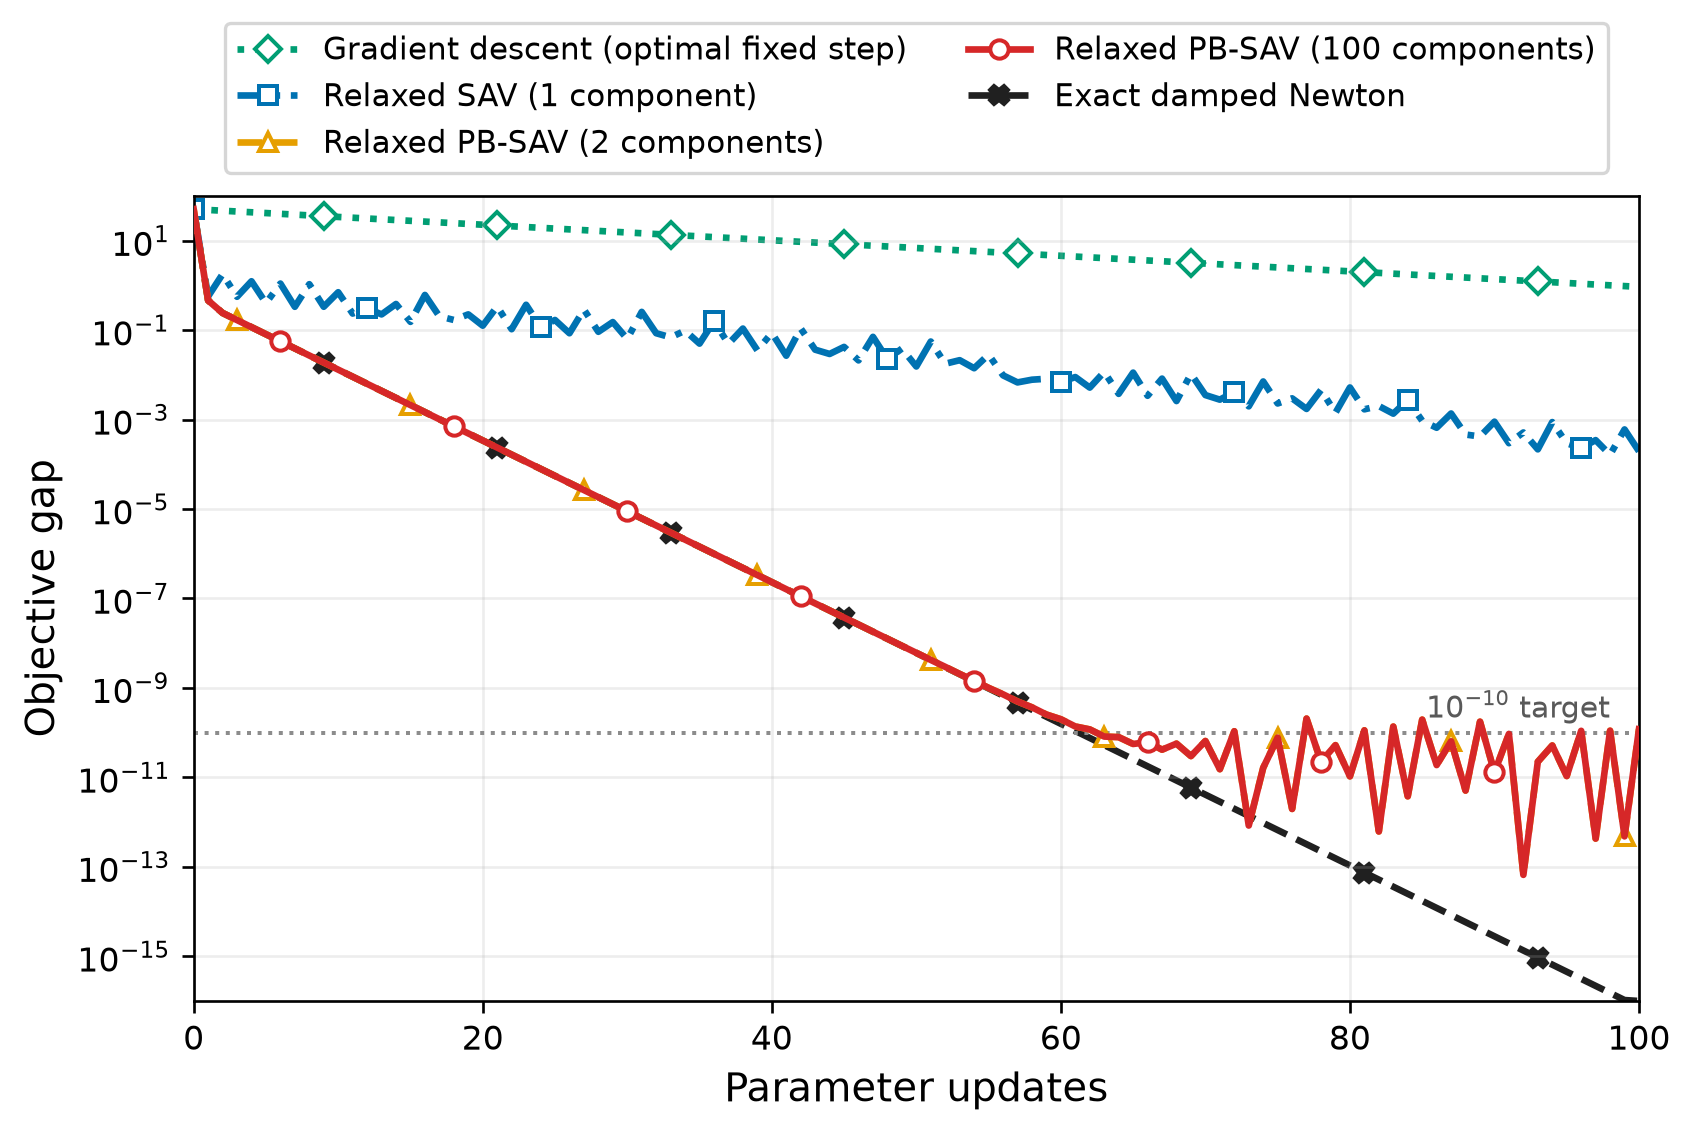
\includegraphics[width=0.78\textwidth]{quadratic_convergence.png}
  \caption{Convergence on the quadratic problem during the first 100 updates.
  All methods start from the same state.}
  \label{fig:quadratic-convergence}
\end{figure}

\begin{figure}[t]
  \centering
  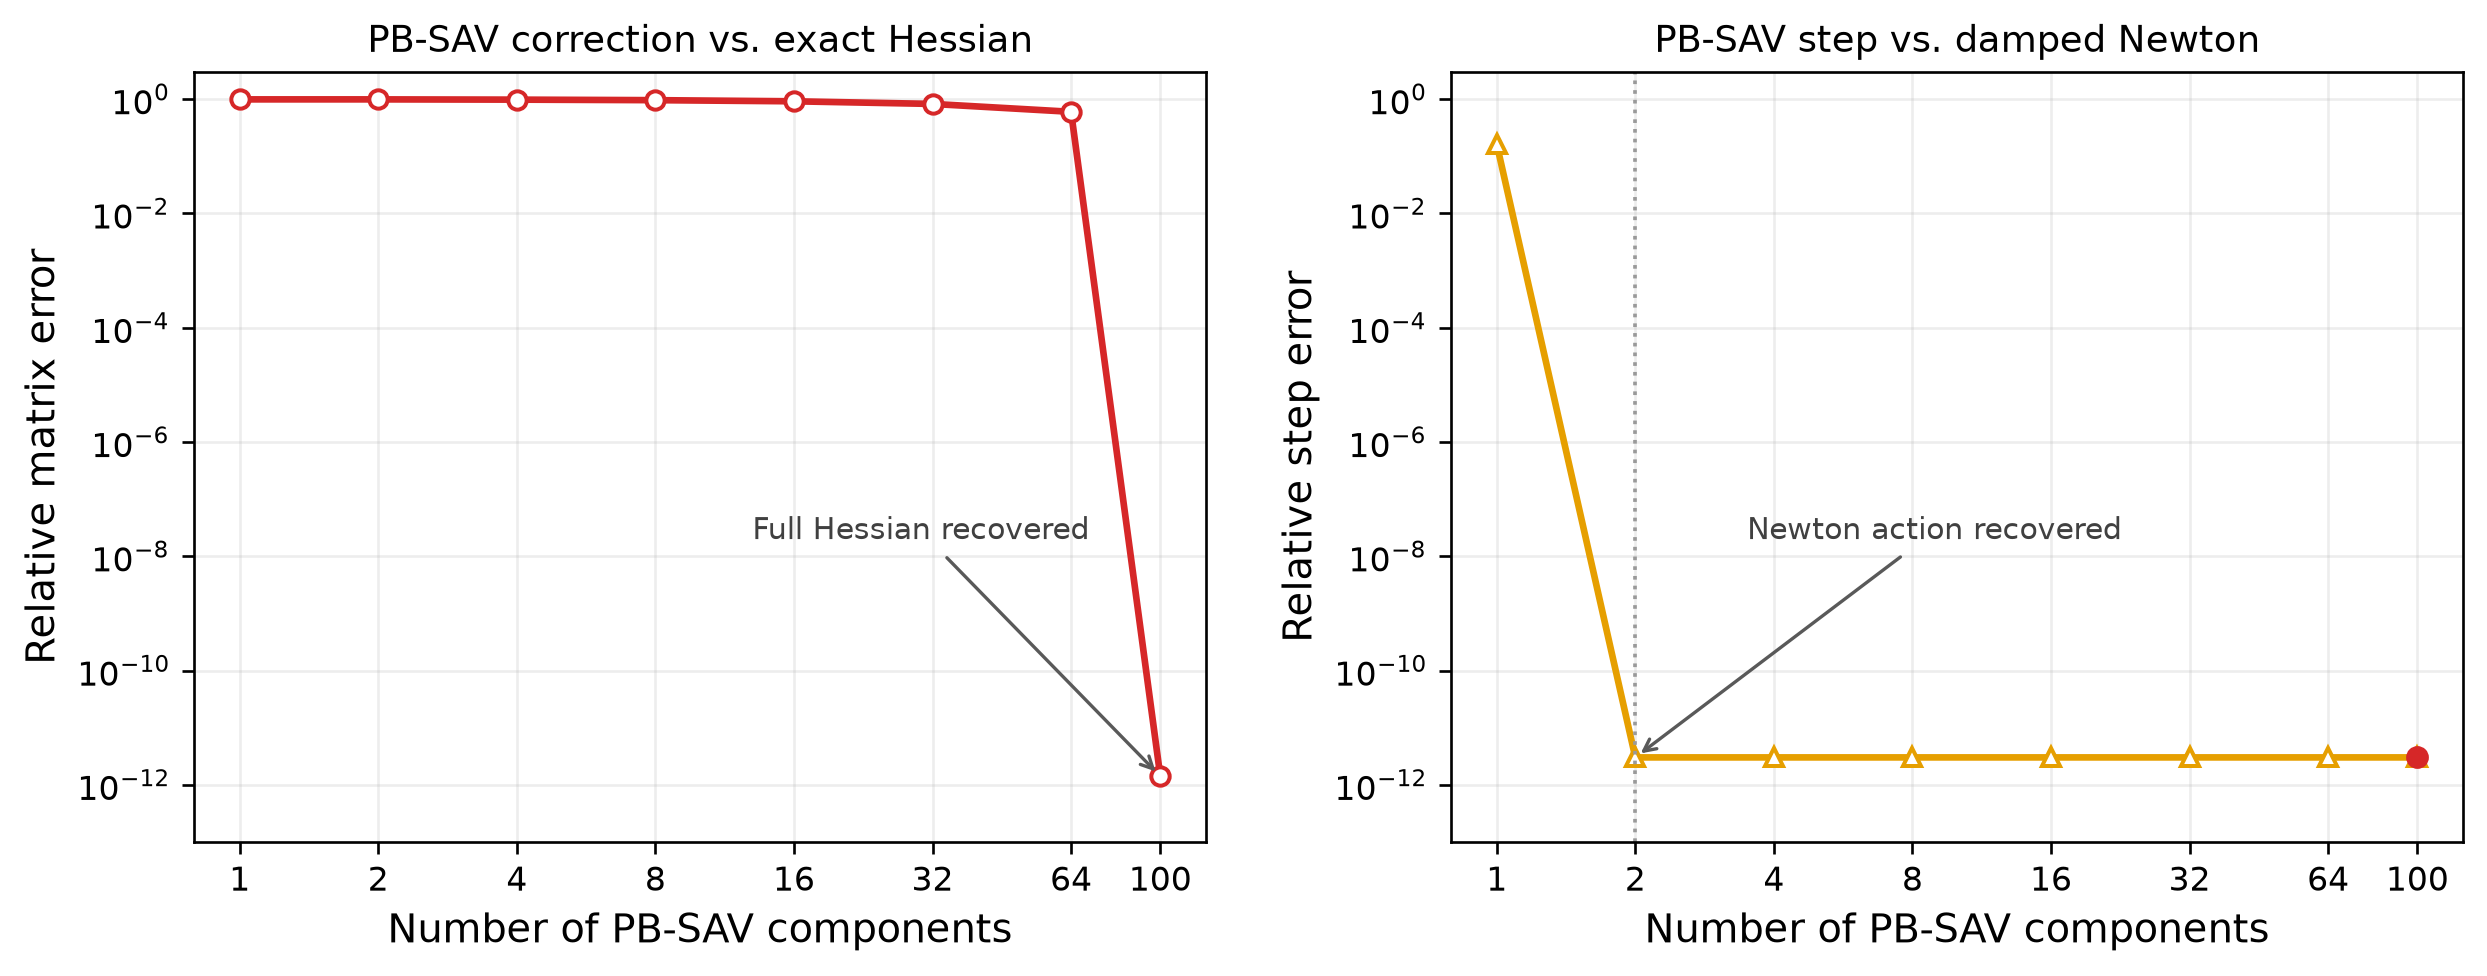
\includegraphics[width=\textwidth]{quadratic_newton_recovery.png}
  \caption{Fixed-state geometry for the quadratic problem.  Left: relative
  error between the PB--SAV correction and the exact Hessian.  Right: relative
  error between the PB--SAV increment and the damped Newton increment.}
  \label{fig:quadratic-recovery}
\end{figure}

\begin{table}[t]
\centering
\caption{Quadratic comparison after 300 updates.  The Hessian and step errors
are evaluated at the common initial state.  The final gap is
\(F(\phi^{300})-F(\phi_*)\), with \(F(\phi_*)=0\).  A dash indicates
that the quantity is not applicable or that the target was not reached within
300 updates.  The columns report different quantities and are not ranked, so no
entry is bold.}
\label{tab:quadratic-results}
\footnotesize
\setlength{\tabcolsep}{2pt}
\begin{tabular}{@{}lcccc@{}}
\toprule
Method & \shortstack{Hessian\\error} & \shortstack{Newton-step\\error} &
\shortstack{Updates to\\\(10^{-10}\)} & \shortstack{Final\\gap} \\
\midrule
Gradient descent (optimal step) & -- & -- & -- & \(3.102\times10^{-4}\) \\
Relaxed SAV (1 comp.) & \(9.900\times10^{-1}\) & \(1.627\times10^{-1}\) & -- & \(1.873\times10^{-10}\) \\
Relaxed PB--SAV (2 comp.) & \(9.899\times10^{-1}\) & \(3.022\times10^{-12}\) & 63 & \(7.879\times10^{-11}\) \\
Relaxed PB--SAV (100 comp.) & \(1.414\times10^{-12}\) & \(3.022\times10^{-12}\) & 63 & \(9.623\times10^{-11}\) \\
Exact damped Newton & -- & 0 & 62 & \(1.550\times10^{-48}\) \\
\bottomrule
\end{tabular}
\end{table}

The fixed-state comparison in \cref{fig:quadratic-recovery} separates the
error in the matrix from the error in the increment it produces.  The
two-component correction has a relative Hessian error of
\(9.899\times10^{-1}\), but its step error is only \(3.022\times10^{-12}\).  The 100-component correction
recovers the full Hessian to \(1.414\times10^{-12}\), yet it produces the same
step accuracy as the two-component formulation.  The trajectories in
\cref{fig:quadratic-convergence,tab:quadratic-results} follow the same
pattern.  The two PB--SAV variants reach the \(10^{-10}\) target in 63
updates, compared with 62 updates for exact damped Newton.  One-component SAV
converges more slowly, and optimally tuned fixed-step gradient descent remains
above the target after 300 updates.

At \(\phi^0\), the gradient lies in the two-dimensional subspace spanned by the
indicator vectors of the two curvature classes.  The two-component pullback
agrees with the damped Hessian on this subspace, but not outside it.

\subsection{Nonlinear regression: Gauss--Newton recovery}
\label{sec:regression-experiment}

The second example tests the pullback interpretation in a nonlinear
least-squares problem.  We fit \(N=30\) noisy observations of
\(f_*(x)=\sin(2\pi x)\) for \(x\in[0,1]\),
where the observation noise is independent Gaussian noise with standard
deviation \(0.1\).  The model is a one-hidden-layer tanh network,
\begin{equation}
  f_\theta(x)=\sum_{j=1}^{50}c_j\tanh(a_jx+b_j)+b_0,
  \label{eq:regression-network}
\end{equation}
with 151 trainable parameters.  The model is therefore overparameterized
relative to the 30 observations.  The objective is
\begin{equation}
  F(\theta)=\frac{1}{2N}\sum_{i=1}^{N}
  \left(f_\theta(x_i)-y_i\right)^2.
  \label{eq:regression-objective}
\end{equation}
For a pointwise least-squares decomposition,
\cref{eq:residual-pullback-curvature} relates the PB--SAV pullback to the
Gauss--Newton matrix, with scaled residuals
\(r_i=(f_\theta(x_i)-y_i)/\sqrt{N}\). This example tests the relation at
both the matrix and trajectory levels.

Nested random partitions use \(1,2,4,8,16\), and 30 components.  The final
partition assigns one squared residual to each observation.  PB--SAV and
damped Gauss--Newton use the same adaptive damping controller, with
\(10^{-6}\leq\eta\leq100\), and the same Armijo acceptance test
\cite{armijo1966} on the true objective. Gradient descent uses the rate
\(0.22\), selected by a paired
200-update training-objective pilot.  Adam is piloted over
\(10^{-3}\), \(3\times10^{-3}\), \(10^{-2}\), and \(3\times10^{-2}\),
and selects \(3\times10^{-2}\).  Each reported run contains 600 accepted
updates.  Prediction is measured by the mean-squared error (MSE) against the
noise-free target.
The PB--SAV runs use the direct update with \(\alpha=1\).

\begin{figure}[t]
  \centering
  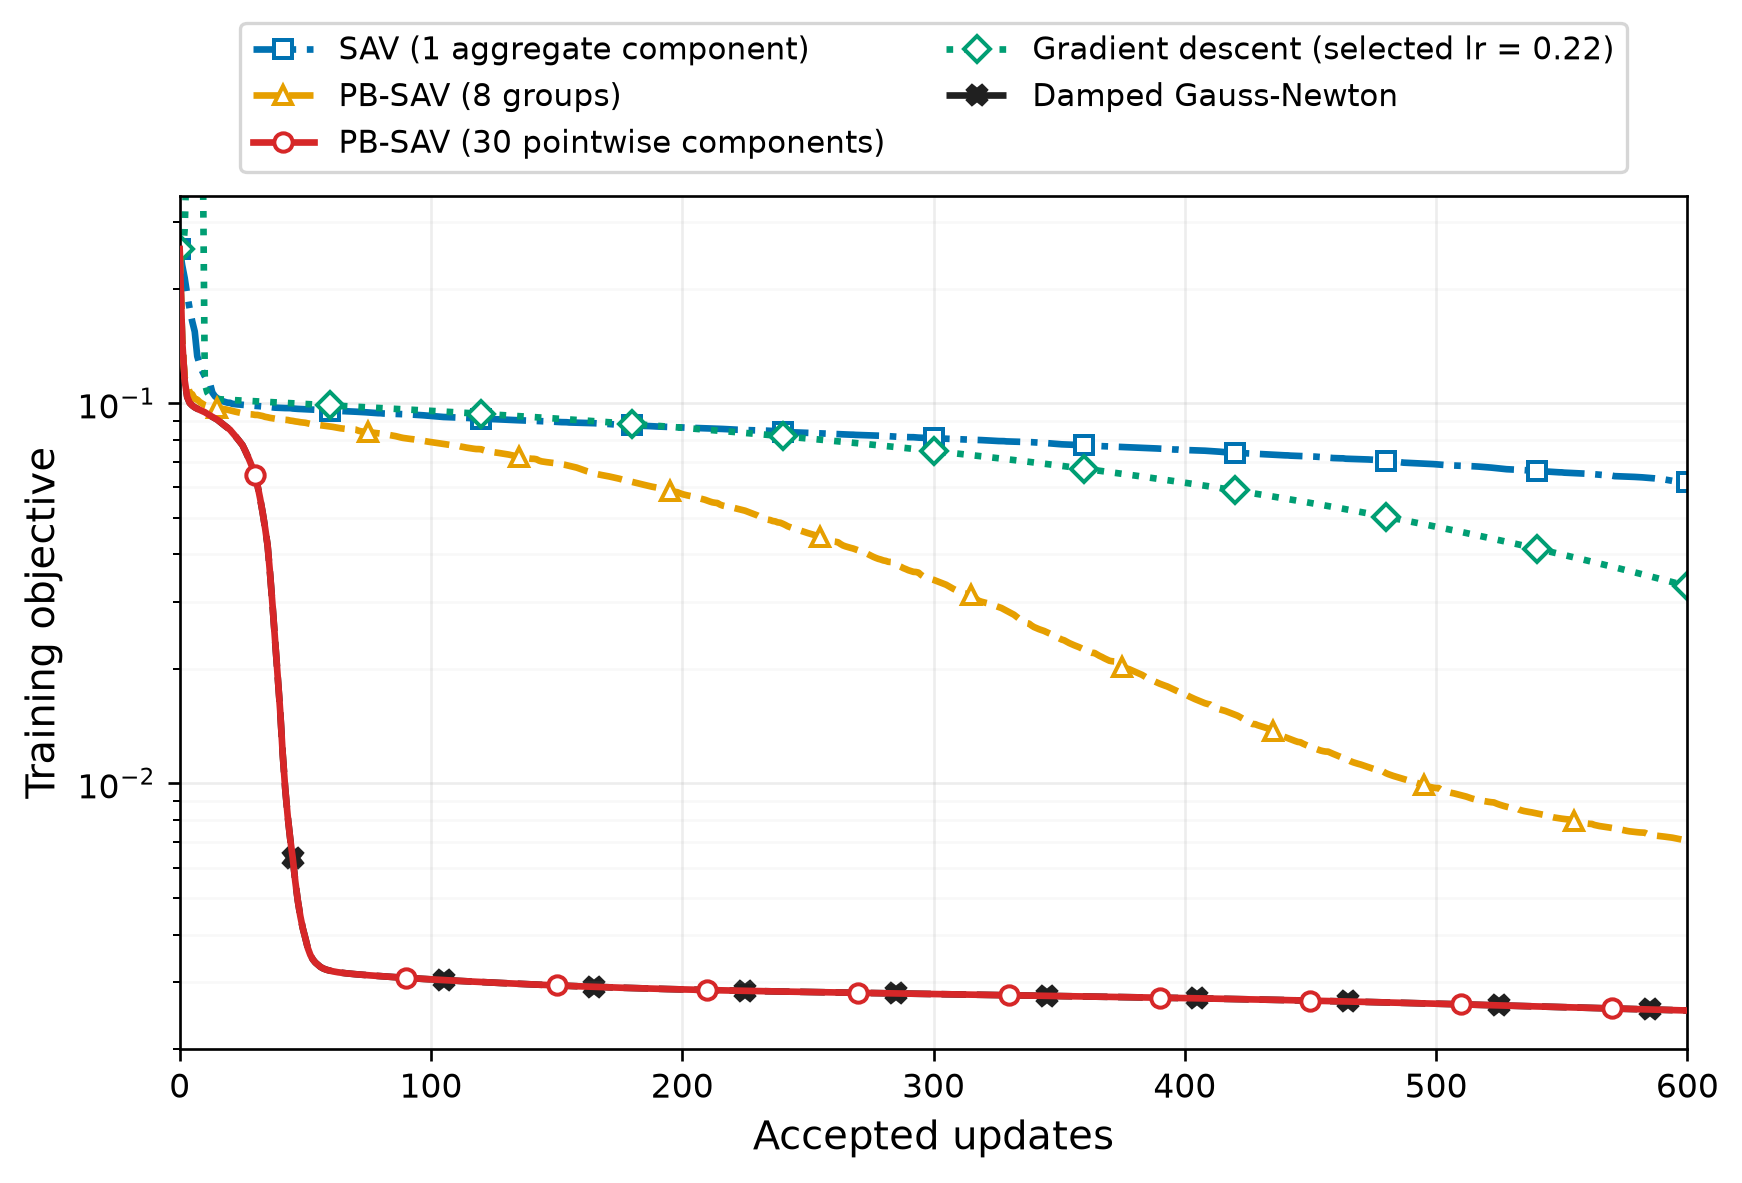
\includegraphics[width=0.80\textwidth]{regression_convergence.png}
  \caption{Training objective for one, eight, and 30 PB--SAV components,
  together with gradient descent and damped Gauss--Newton.  The pointwise
  PB--SAV and Gauss--Newton trajectories are indistinguishable at plotting
  resolution.}
  \label{fig:regression-convergence}
\end{figure}

\begin{figure}[t]
  \centering
  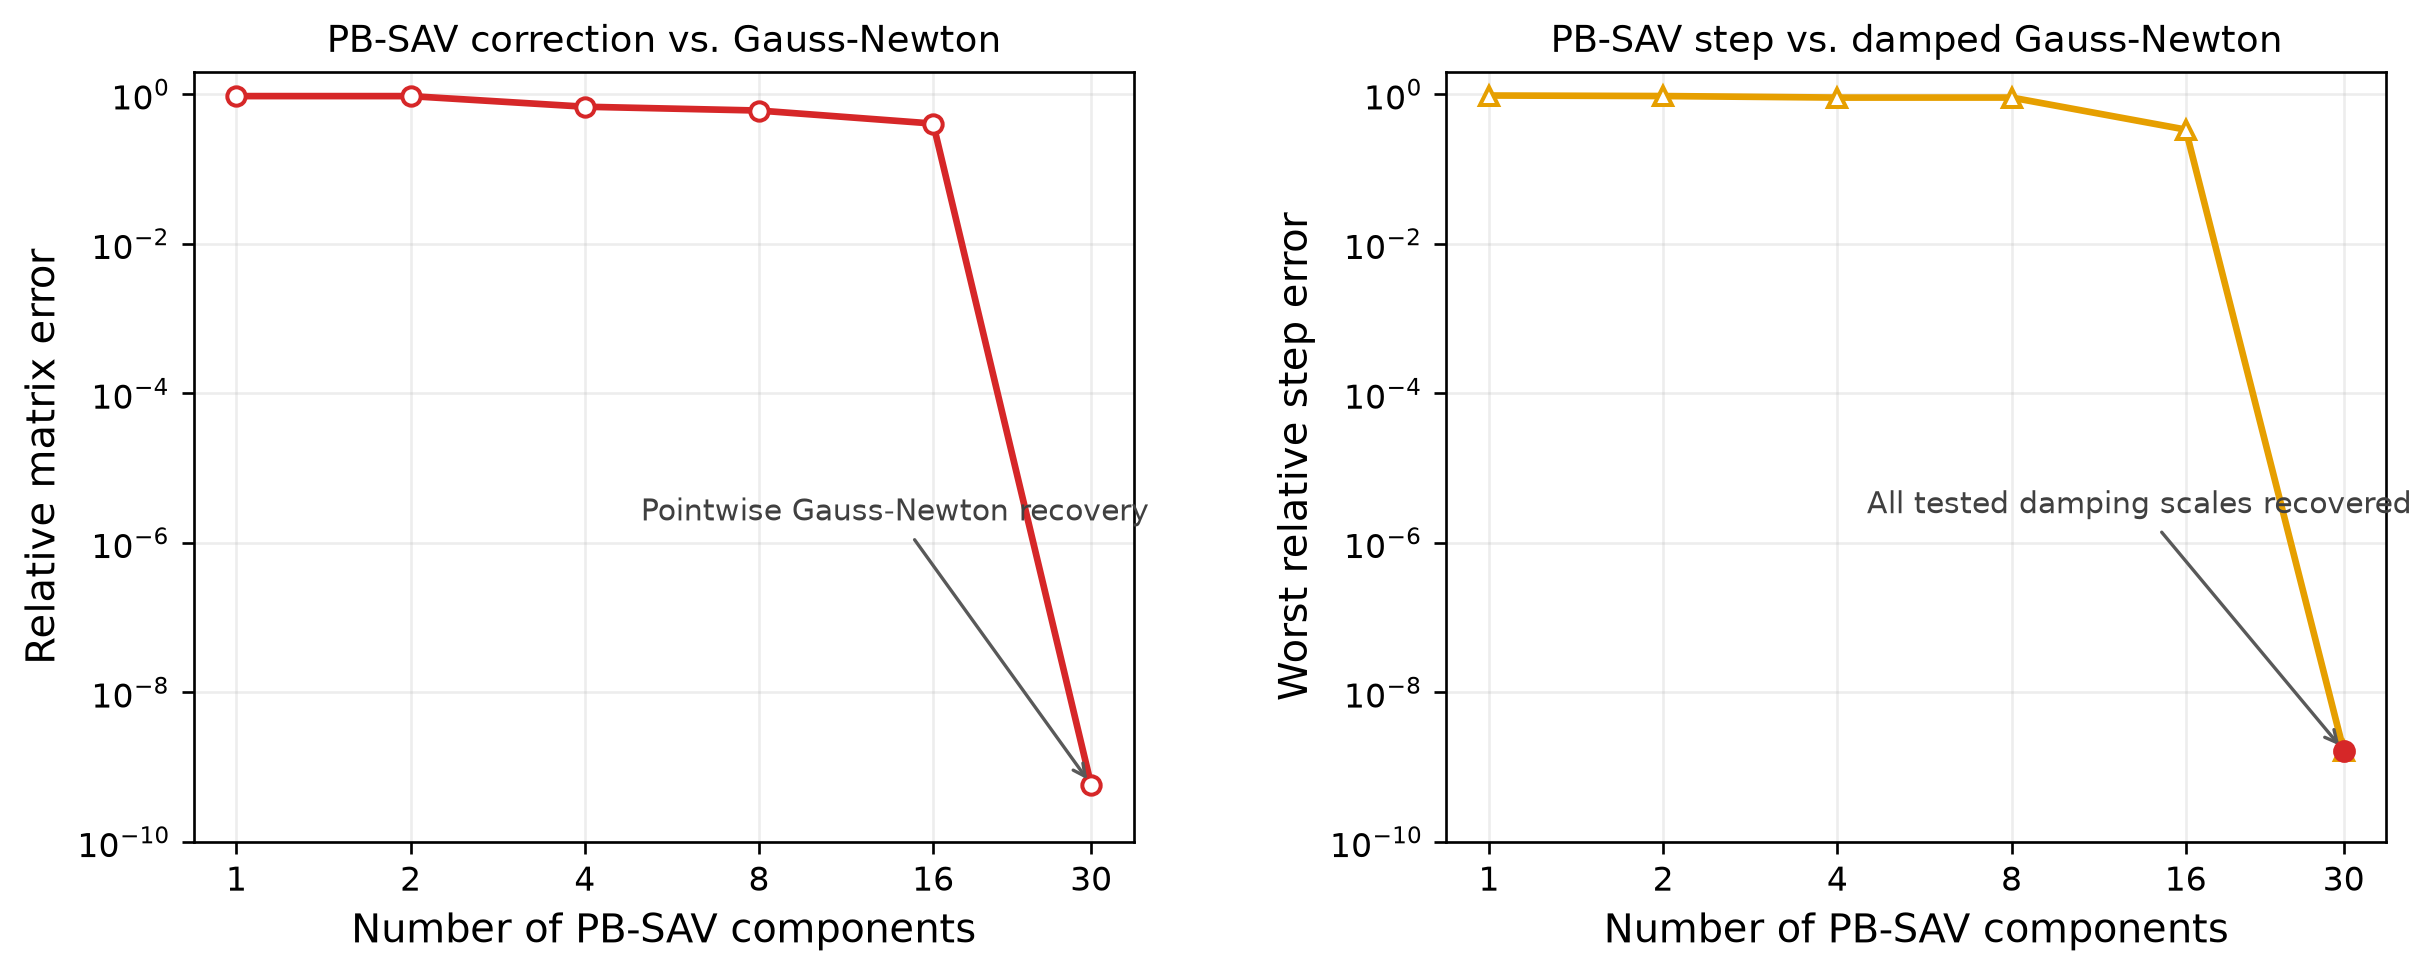
\includegraphics[width=\textwidth]{regression_gauss_newton_recovery.png}
  \caption{Fixed-state geometry for nonlinear regression.  Left: relative
  error between the PB--SAV correction and the Gauss--Newton matrix.  Right:
  the largest relative step error over \(\eta=0.1,1,10,100\).  Both errors
  collapse when each observation is represented by a separate component.}
  \label{fig:regression-recovery}
\end{figure}

\begin{table}[t]
\centering
\caption{Nonlinear-regression results after 600 accepted updates.  No entry is
bold: PB--SAV and damped Gauss--Newton agree in every column to the displayed
precision.}
\label{tab:regression-results}
\footnotesize
\setlength{\tabcolsep}{3pt}
\begin{tabular}{@{}lcccc@{}}
\toprule
Method & Updates & \shortstack{Final\\objective} &
\shortstack{Best noise-free\\test MSE} & \shortstack{Final\\\(\|\nabla F\|\)} \\
\midrule
PB--SAV (30 pointwise comp.) & 600 & \(2.525\times10^{-3}\) & \(2.804\times10^{-3}\) & \(1.032\times10^{-4}\) \\
Damped Gauss--Newton & 600 & \(2.525\times10^{-3}\) & \(2.804\times10^{-3}\) & \(1.032\times10^{-4}\) \\
Gradient descent (rate 0.22) & 600 & \(3.301\times10^{-2}\) & \(6.040\times10^{-2}\) & \(2.468\times10^{-2}\) \\
Adam & 600 & \(2.985\times10^{-3}\) & \(3.113\times10^{-3}\) & \(6.695\times10^{-4}\) \\
\bottomrule
\end{tabular}
\end{table}

\Cref{fig:regression-convergence} shows the trajectories and
\cref{fig:regression-recovery} the fixed-state errors.
At the common initial state, the pointwise PB--SAV correction differs from the
Gauss--Newton matrix by only \(5.82\times10^{-10}\).  The relative step errors
for \(\eta=0.1,1,10,100\) are \(2.31\times10^{-10}\),
\(3.71\times10^{-10}\), \(9.72\times10^{-10}\), and \(1.67\times10^{-9}\),
and the direction cosine equals one to displayed precision in every case.
The effective correction rank is 17 rather than the nominal 30, consistent
with the rank of the sample Jacobian at the initial state.  Along the full
trajectory, pointwise PB--SAV and damped Gauss--Newton agree in final objective
to \(1.24\times10^{-11}\).  They also attain the same noise-free test MSE and final
gradient norm in \cref{tab:regression-results}.

The pointwise components expose the individual residual Jacobians, so the
PB--SAV correction reproduces the Gauss--Newton geometry up to the small shift
regularization. Coarser partitions aggregate these directions before forming
the pullback.

\subsection{Operator learning: two-dimensional Darcy flow}
\label{sec:darcy-experiment}

We next apply PB--SAV with separate components for the supervised data loss
and weight decay to operator learning and compare it with heavy-ball gradient descent and
AdamW. For each
permeability field \(a(x,y)\), the target solution satisfies
\begin{equation}
  -\nabla\!\cdot\!\left(a(x,y)\nabla u(x,y)\right)=1,
  \qquad (x,y)\in\Omega=(0,1)^2,
  \qquad u|_{\partial\Omega}=0.
  \label{eq:darcy-problem}
\end{equation}
The permeability is generated by thresholding a smoothed Gaussian random
field with correlation length \(0.12\), which produces the two values 3 and
12.  Finite-difference solutions are represented on a \(33\times33\) grid.
For each seed, the dataset contains 128 training functions and 64 independently
generated test functions.

We use a 51,521-parameter convolutional-branch deep operator network
(DeepONet) \cite{lu2021deeponet}. The branch encoder uses convolutional channel widths
\(8,16,32\), adaptive \(4\times4\) pooling, and a 64-dimensional projection.
The trunk is a three-hidden-layer tanh network of width 64 and maps spatial
coordinates to the same latent dimension.  Multiplication by
\(16x(1-x)y(1-y)\) enforces the homogeneous Dirichlet boundary condition exactly.

Let \(N_{\rm tr}=128\) and \(N_x=33^2\).  For training field \(a_j\), let
\(u_j(x_\ell)\) be the reference solution at grid point \(x_\ell\), and let
\(\widehat u_\theta(a_j;x_\ell)\) be the network prediction.  Define
\begin{align}
  E_{\rm data}(\theta)
  &=\frac{1}{2N_{\rm tr}N_x}
    \sum_{j=1}^{N_{\rm tr}}
    \sum_{\ell=1}^{N_x}
    \left(\widehat u_\theta(a_j;x_\ell)-u_j(x_\ell)\right)^2,\\
  E_{\rm wd}(\theta)
  &=\frac{\lambda}{2}\norm{\theta}^2,
  \qquad \lambda=3\times10^{-5},
\end{align}
PB--SAV uses the two-component objective
\begin{equation}
  F_{\rm Darcy}(\theta)=E_{\rm data}(\theta)+E_{\rm wd}(\theta).
  \label{eq:darcy-objective}
\end{equation}
The common training quantity reported here is \(E_{\rm data}\).
Generalization is measured by the relative \(L^2\) error on the held-out
operator dataset.

The selected learning rates are \(10^{-2}\), \(10^{-3}\), and
\(3\times10^{-3}\) for heavy-ball gradient descent, AdamW, and PB--SAV,
respectively. PB--SAV uses \(\beta=0.9\),
\(\beta_2=0.999\), \(\epsilon=10^{-8}\), \(\alpha=0.5\), and
\(\rho^n\equiv1\). These PB--SAV parameters are also used in the following Burgers experiments unless otherwise stated.  Each
method runs for 5,000 full-batch updates using the paired seeds
\(42, 101, 211, 307, 401\).
The displayed field is the fixed test sample with the greatest variation in
the reference solution.

\begin{figure}[t]
  \centering
  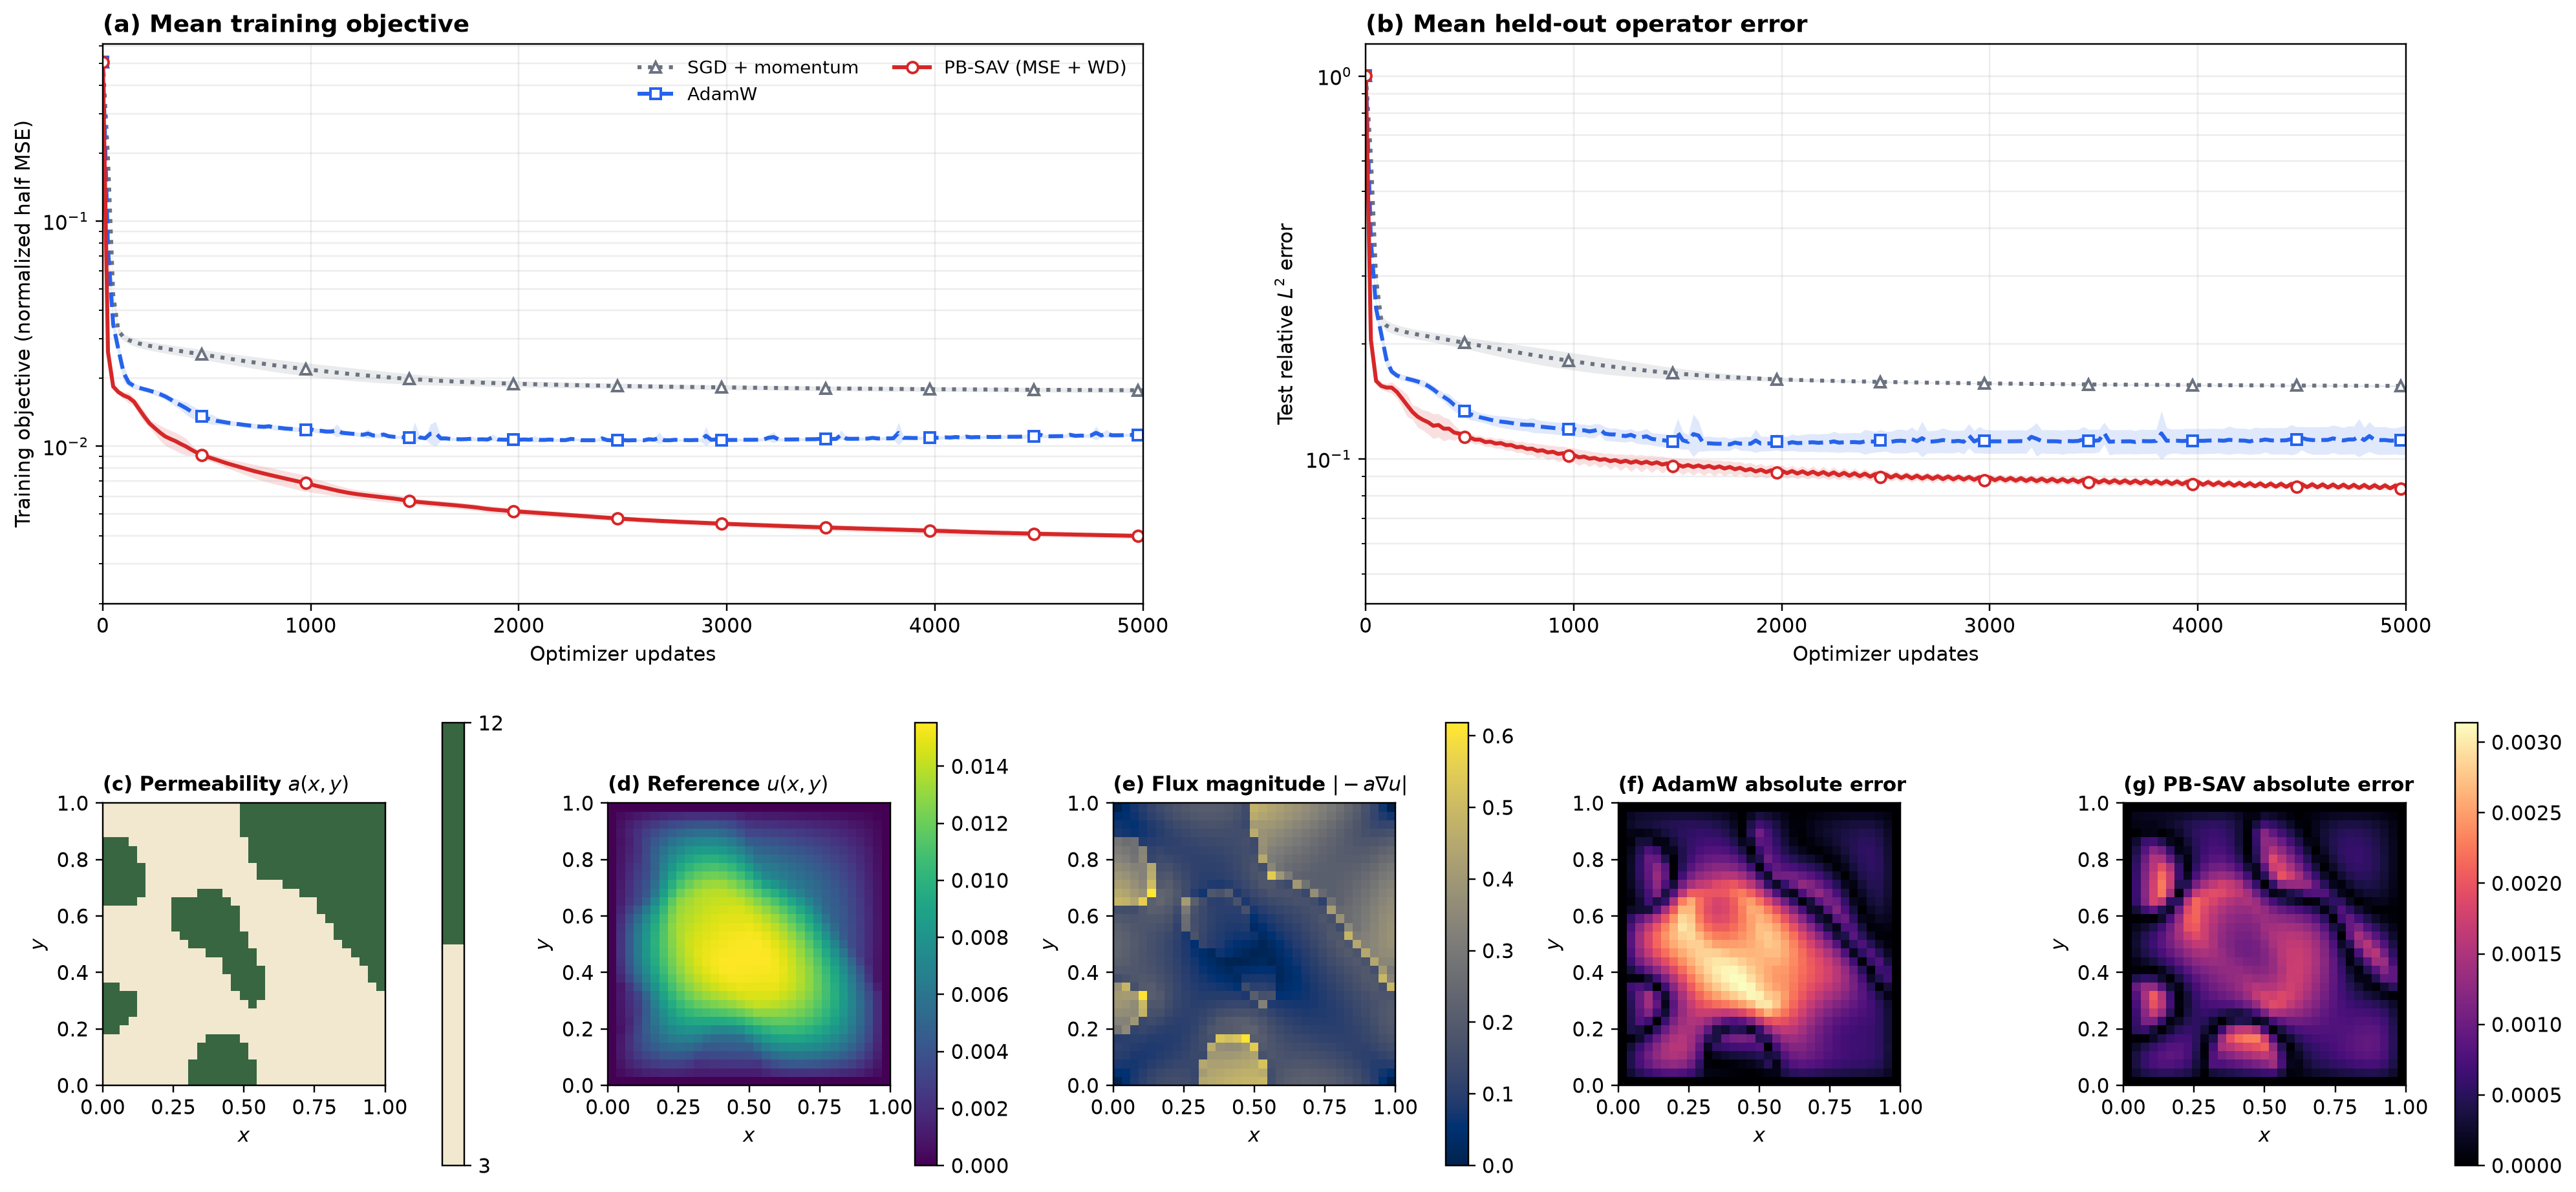
\includegraphics[width=\textwidth]{darcy_deeponet_screen_comparison.png}
  \caption{Five-seed Darcy DeepONet comparison.  (a) Mean common training data
  loss and (b) mean held-out relative \(L^2\) error; shaded regions show one
  sample standard deviation.  The legend entry ``SGD + momentum'' in (a) and
  (b) is the full-batch heavy-ball gradient descent of \cref{tab:darcy-results}.  The lower row shows a fixed test sample selected
  by the maximum variation of the reference field: (c) permeability, (d) reference
  solution, (e) flux magnitude, (f) AdamW absolute error, and (g) PB--SAV
  absolute error.}
  \label{fig:darcy-results}
\end{figure}

\begin{table}[t]
\centering
\caption{Darcy DeepONet results after 5,000 updates over five paired seeds.
Losses and errors are reported as mean \(\pm\) sample standard deviation.  Wall
time is the mean recorded time for the full training run.  Best mean training
and test values are bold; wall time is reported for reference and is not
ranked.}
\label{tab:darcy-results}
\scriptsize
\setlength{\tabcolsep}{3pt}
\begin{tabular}{@{}lccccc@{}}
\toprule
Method & Components & \(\eta\) & \shortstack{Train data\\loss} &
\shortstack{Test relative\\\(L^2\)} & \shortstack{Wall time\\(s)} \\
\midrule
\shortstack[l]{Heavy-ball\\gradient descent} & -- & \(10^{-2}\) & \(0.01771\pm0.00041\) & \(0.15510\pm0.00095\) & 37.4 \\
AdamW & -- & \(10^{-3}\) & \(0.01125\pm0.00024\) & \(0.11264\pm0.01001\) & 36.5 \\
\shortstack[l]{PB--SAV (data +\\weight decay)} & 2 & \(3\times10^{-3}\) & \(\mathbf{0.00399\pm0.00011}\) & \(\mathbf{0.08512\pm0.00225}\) & 74.5 \\
\bottomrule
\end{tabular}
\end{table}

PB--SAV attains the lowest training and test errors in
\cref{fig:darcy-results,tab:darcy-results}.  Relative to AdamW, it reduces the
mean training data loss by 64.5\% and the mean held-out error by 24.4\%.
Relative to heavy-ball gradient descent, the reductions are 77.5\% and
45.1\%, respectively.
The standard deviation of the PB--SAV test error is \(0.00225\), compared with
\(0.01001\) for AdamW.  In the lower row of \cref{fig:darcy-results}, the PB--SAV prediction has a
smaller error over most of the domain for the displayed test sample.

With two components, PB--SAV gives lower mean training and test errors than
the two baselines at approximately twice the recorded wall time of AdamW.
This comparison evaluates the complete optimizer. The following forward
Burgers experiment includes a one-component PB--SAV baseline to examine the
effect of the decomposition itself.
